\begin{figure}[H]
  \centering

  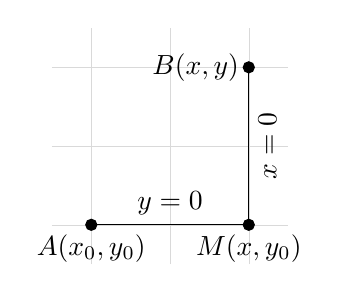
\begin{tikzpicture}
    \draw[very thin, gray!30, step = 1cm] (0.5, 0.5) grid (3.5, 3.5);
    
    \draw[fill = black] (1, 1) circle (2pt);
    \draw node[below] at (1, 1) {\(A(x_{0}, y_{0})\)};
  
    \draw[fill = black] (3, 1) circle (2pt);
    \draw node[below] at (3, 1) {\(M(x, y_{0})\)};
  
    \draw[fill = black] (3, 3) circle (2pt);
    \draw node[left] at (3, 3) {\(B(x, y)\)};
  
    \draw (1, 1) -- (3, 1)
      node[midway, above] {\(\dd y = 0\)};
    \draw (3, 3) -- (3, 1)
      node[midway, below, sloped, rotate = 180] {\(\dd x = 0\)};
  \end{tikzpicture}  
\end{figure}